\section{Introduction}

In the MIPS32 architecture, all machine instructions are represented
as 32-bit numbers. This article presents a MIPS32-decompiler that,
when passed 32-bit numbers which either partially or completely
represent MIPS32 instructions yields a series of different
representations of the same instruction.

Specifically, MIPS32 instructions are to be read from a file with
numbers either in decimal or hexadecimal form. For each number in the
input file, the disassembler will produce the following:

\begin{itemize}
  \item The number from the input file.
  \item The format of the instruction (R, I, or J).
  \item The decomposed representation in decimal.
  \item The decomposed representation in hexadecimal.
  \item The representation of the instruction in mnemonic format,
    using register abbreviations wherever possible (e.g.,
    \texttt{\$t0} instead of \texttt{\$8}) and using decimal numbers
    whenever actual numbers are necessary.
\end{itemize}

In the following subsections an introduction of the terminology used
throughout this document is provided. Afterwards you may refer to this
section again if any of the above requirements seem foreign to you.

The rest of the document will be dedicated to a high-level description
of this solution accompanied with a guide on how to compile and run
the software.

The appendix contains an overview of all those instructions that the
decompiler is capable of comprehending.

\subsection{Terminology}

% TODO: cite
According to Aho et al.  a \emph{compiler} is a program that
can read a program in one language --- the \emph{source} language --
and translates it into an equivalent program in another language --
the \emph{target} language; see Fig. \ref{fig:compiler}.

\begin{figure}[H]
  \centering
  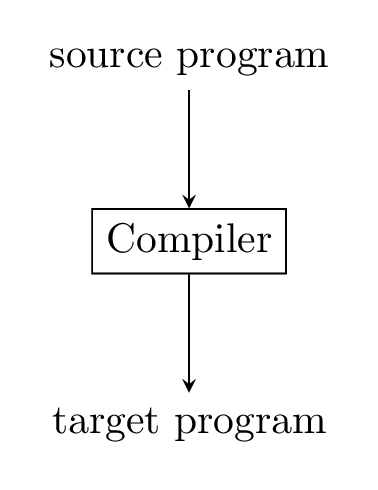
\includegraphics[width=0.3\textwidth]{figures/compiler.png}
  \caption{A compiler}
  \label{fig:compiler}
\end{figure}

Conversely, a \emph{decompiler} is also a that performs the reverse
operation of a compiler. It too, is a compiler. Commonly one views a
compiler as a translator from a high-level human-readable source
language into a low-level machine-readable language, similarly a
decompiler translates in the opposite direction; see
Fig. \ref{fig:decompiler}. 

The two exhibit a chiral relation to one another, i. e. that they are
mirrored images of each other in terms of functionality, but they are
not themselves identical.

\begin{figure}[H]
  \centering
  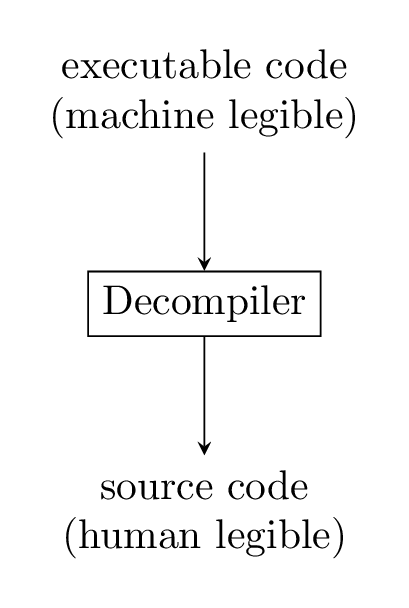
\includegraphics[width=0.3\textwidth]{figures/decompiler.png}
  \caption{A decompiler}
  \label{fig:decompiler}
\end{figure}

In this assignment the decompiler must be able to translate from the
machine-readable language of 32-bit numbers representing MIPS32
instructions to the human-readable target language described in the
introduction.

By example, the constituent parts of the decompilers output will
be described further.

Specifically,

\begin{itemize}
  \item Format.
  \item Opcode.
  \item Decomposed representation.
  \item Mnemonic representation.
\end{itemize}

will be covered.

Consider the 32-bit number \texttt{0x71014802}. It is \emph{decomposed}
into fields of varying lengths depending on the \emph{format} of the
instruction.

For all numbers in the MIPS32 instruction set the leftmost six bits
always represent the opcode for the instruction. The opcode alone is
not always sufficient to identify the particular instruction,
\emph{but} it is always sufficient to identify the format of the
instruction.

The leftmost six bits of \texttt{0x71014802} is \texttt{0x1c}. It is
\emph{known} that this number corresponds to an instruction in the
R-format. The format specifies into which fields the remaining bits
decompose into. In Fig. \ref{fig:r-decomposed} each field's size in
bits is the small number below the field.

\begin{figure}[H]
  \centering
  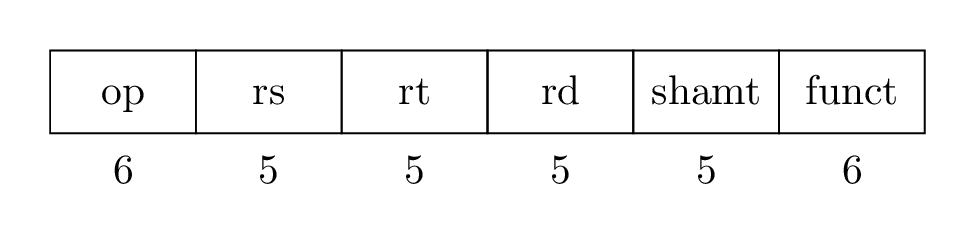
\includegraphics[width=0.9\textwidth]{figures/r-decomposed.png}
  \caption{The fields of an R-type instruction}
  \label{fig:r-decomposed}
\end{figure}

This subsection concludes with a concept review that serves as a brief
summary for the reader.

\subsection{Problem statement}


In this assignment the core functionality which is exposed is
\emph{parsing} such a number and outputting other representations of
the same instruction, as well as some additional information regarding
it.

\subsection{Concept review}
